\chapter{Introduction}

\chapter{CellBE platform}

This chapter will introduce Cell Broadband Engine processor (CellBE) and the whole platform and its specifics.

\section{About the processor}

CellBE processor is representative of a new generation of IBM's CellBE platform family made by collaboration of IBM, Sony, and Toshiba.
CellBE is an asymmetric, high-performance multi-core processor that combines eight synergistic processing elements (SPEs) and a Power Processing Element (PPE), which is a general-purpose IBM \textregistered{PowerPC} core.
Next part is a central memory element.
PPE can operate with the central memory directly while SPE indirectly, see below.
In CellBE is several kinds memoreis.
All the elements are connected through high speed bus (EIB - Element Interconnect Bus).
Whole layout is on figure \ref{fg:processorLayout}.

\begin{figure}
    \centering
    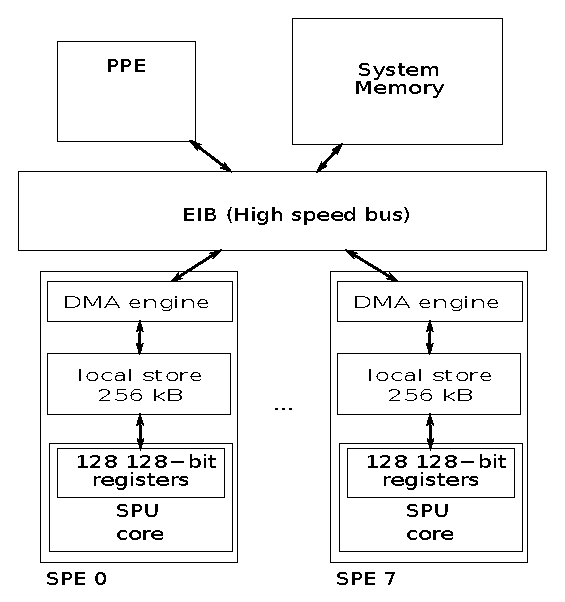
\includegraphics[width=\textwidth]{data/cellLayout}
    \caption[CellBE processor layout]{One PPE unit along with eight SPE stream processor units and system memory connected together with high speed EIB bus}
    \label{fg:processorLayout}
\end{figure}

Each SPE has a 4-way SIMD unit, a high-speed private local store memory and a direct memory access (DMA) engine.
The SIMD unit has 128 128-bit wide general purpose regiters.
Vectorized oprations in various data types configurations can be performed with these registers.
E.g. two double-precision floats or 8 32bit integers can be processed at single clock tick.
Unlike conventional microprocessors, SPE does not have a hardware cache.
Its function supply the small on-chip local store memory under programmer's control.
This allow code optimizations that can reduce cache misses.
The local store is separated from the main memory (on which the PPE operates), so SPE has its own address space.
Therefore any synchronization with other cores is not neccessary.
The local store is attached to a larger (central) shared memory through DMA engine that
manages transfering data from central memory to local store and vice versa.
Therefore, this CellBE can be viewed as a distributed memory multiprocessor.

CellBE achieves a significant performance per Watt and performance per chip area advantage over conventional high-performance processors.
Is significantly more flexible and programmable than single-function and other optimized processors such as graphics processors, or conventional digital signal processors.
While a conventional microprocessor may deliver about 20+GFlops of single-precision (32b) floating-point performance, Cell delivers 200+ GFlops (in ideal conditions) at comparable power.

A number of signal processing and media applications have been implemented on Cell with excellent results.
Advanced visualization such as ray-casting, ray-tracing, and volume rendering.
Streaming applications such as media encoders and decoders and streaming encryption and decryption standards have also been demonstrated to perform about an order of magnitude better on Cell than on conventional PC.

\subsection{PPE - \textregistered{PowerPC} Processing Element}
PPE is derived from IBM \textregistered{PowerPC} core. Has 512kB L2 cache on die.
It supports the Power Architecture ISA, inherits the memory translation, protection, and SMP coherence model of mainstream 64-bit Power processors.
CBEA also supports virtualization (logical partitioning), large pages, and other recent innovations in the Power architecture.
Programming for the PPE is the same as for conventional processors due to direct access to central memory.

\subsection{SPE - Synergistic Processing Element}
SPE is an autonomous processor (sometimes called accellerator) targeted for computational intensive applications.
It supports a SIMD-RISC instruction set.
Has 128 (128-bit long) unified registers to store all types of data (in contrast from traditional RISCs where registers are devided according data types).
One of CellBE programming aspects is converting the code that it uses the SIMD instructions.
This process is calleed "SIMDation".

SPE stores its program and data in its associated local storage memory as private memory.
DMA transactions are used to tranfer data from/to central memory as well as between two local stores.
We say that data is "DMAed" from source to destination.
DMA commands can be issued in many ways.
Synchronous, asynchronous, in scatter-gaether manner through DMA lists.
This memory management is another big part of programming for CellBE.

Programming for SPE has some differencies over programming for conventional processor.
Programmer have always to count with the fact that have only 256kB for the program and data.

This processor is embeded in Sony Playstation 3 game console as well as IBM Blade servers where two or more such processors (as building blocks) connected by high speed bus creates powerfull and modular machine.
We have PlayStation3 machine available for this work.